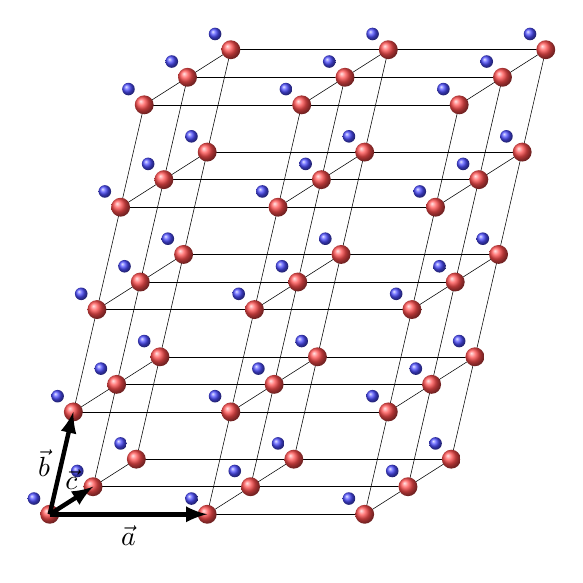
\begin{tikzpicture}[x  = {(1cm,0cm)},
  y  = {(0cm,1cm)},
  z  = {(0.35cm,0.35cm)},
  scale = 1]

  % angle
  % \filldraw[fill=red!35,draw=red!45,opacity=0.5]
  % (3,0.5) -- (1,0.5) arc (180:147:2) -- cycle;
  % \draw (1.75,0.6) node[above] {$\theta$};

  % grid
  % \draw[style=help lines,color=red!45][step=0.5cm] (-0.4,0.1) grid (6.4,2.4);
  % \draw[color=red!70, thick] (-0.4,0.5) -- (6.4,0.5);
  % \draw[->, >=latex, color=red!70, thick] (3,0.1) -- (3,3) node[left] {$\bf h$};

  \def\dax{2}
  \def\day{0.3}
  \def\daz{0.2}
  \def\dby{1.3}

  % grid
  \foreach \y in {0,1,...,4}
  \foreach \z in {0,1,...,2}
  \draw[style=help lines,color=black] (\dax*0+\day*\y+\daz*\z,\dby*\y,\z)
  -- (\dax*2+\day*\y+\daz*\z,\dby*\y,\z);

  \foreach \x in {0,1,...,2}
  \foreach \z in {0,1,...,2}
  \draw[style=help lines,color=black] (\dax*\x+\day*0+\daz*\z,\dby*0,\z)
  -- (\dax*\x+\day*4+\daz*\z,\dby*4,\z);

  \foreach \x in {0,1,...,2}
  \foreach \y in {0,1,...,4}
  \draw[style=help lines,color=black] (\dax*\x+\day*\y+\daz*0,\dby*\y,0)
  -- (\dax*\x+\day*\y+\daz*2,\dby*\y,2);

  % path to vector h
  % \draw[->, >=latex, ultra thick, color=green, style=dashed] (0,0,0) ->
  % +(\dax*3,0,0) -> +(\dax*3+\daz*1,0,1) -> (\dax*3+\day*2+\daz*1,\dby*2,1);

  % atoms
  \foreach \x in {0,1,...,2}
  \foreach \y in {0,1,...,4}
  \foreach \z in {0,1,...,2}
  {
  \shade[ball color=red!70] (\dax*\x+\day*\y+\daz*\z,\dby*\y,\z) circle (.12cm);
  \shade[ball color=blue!70] (\dax*\x+\day*\y+\daz*\z-0.2,\dby*\y+0.2,\z) circle (.08cm);
  }

  % unit cell
  \draw[->, >=latex, ultra thick] (0,0,0) -> node[left] {$\vec{b}$}
  (\day,\dby,0);
  \draw[->, >=latex, ultra thick, color=black]
  (0,0,0) -> node[below] {$\vec{a}$} (\dax,0,0);
  \draw[->, >=latex, ultra thick, color=black]
  (0,0,0) -> node[above] {$\vec{c}$} (\daz,0,1);

  % vector
  % \draw[->, >=latex, thick] (0,0,0) -> node[above] {$\vec h$}
  % (\dax*3+\day*2+\daz*1,\dby*2,1);
\end{tikzpicture}

%%% Local Variables:
%%% mode: latex
%%% TeX-master: "ChapterOne"
%%% End:
